\begin{minipage}{0.63\textwidth}
    \parskip=1em
    \section*{セキュリティモジュール:音楽記号}
    
    \uline{概要}:音楽記号が書かれている5つの板とその上にモールス符号が書かれた紙があります。記号は上下の矢印を使用して変更できます。
\end{minipage}%
\hfill%
\begin{minipage}{0.33\textwidth}
    
\includegraphics[width=\textwidth]{images/54.png}
    \vspace*{\fill}
\end{minipage}
    
\uline{解除方法}:各板を正しい音楽記号に設定します。\\付録IIIを参照して各モールス符号を文字または数字に変換します。次に{、}この文字または数字を下で見つけて{、}対応する記号を設定します。

モジュールは{、}5つの記号すべてに正しく設定してから3秒後に解除されます。

\begin{center}
    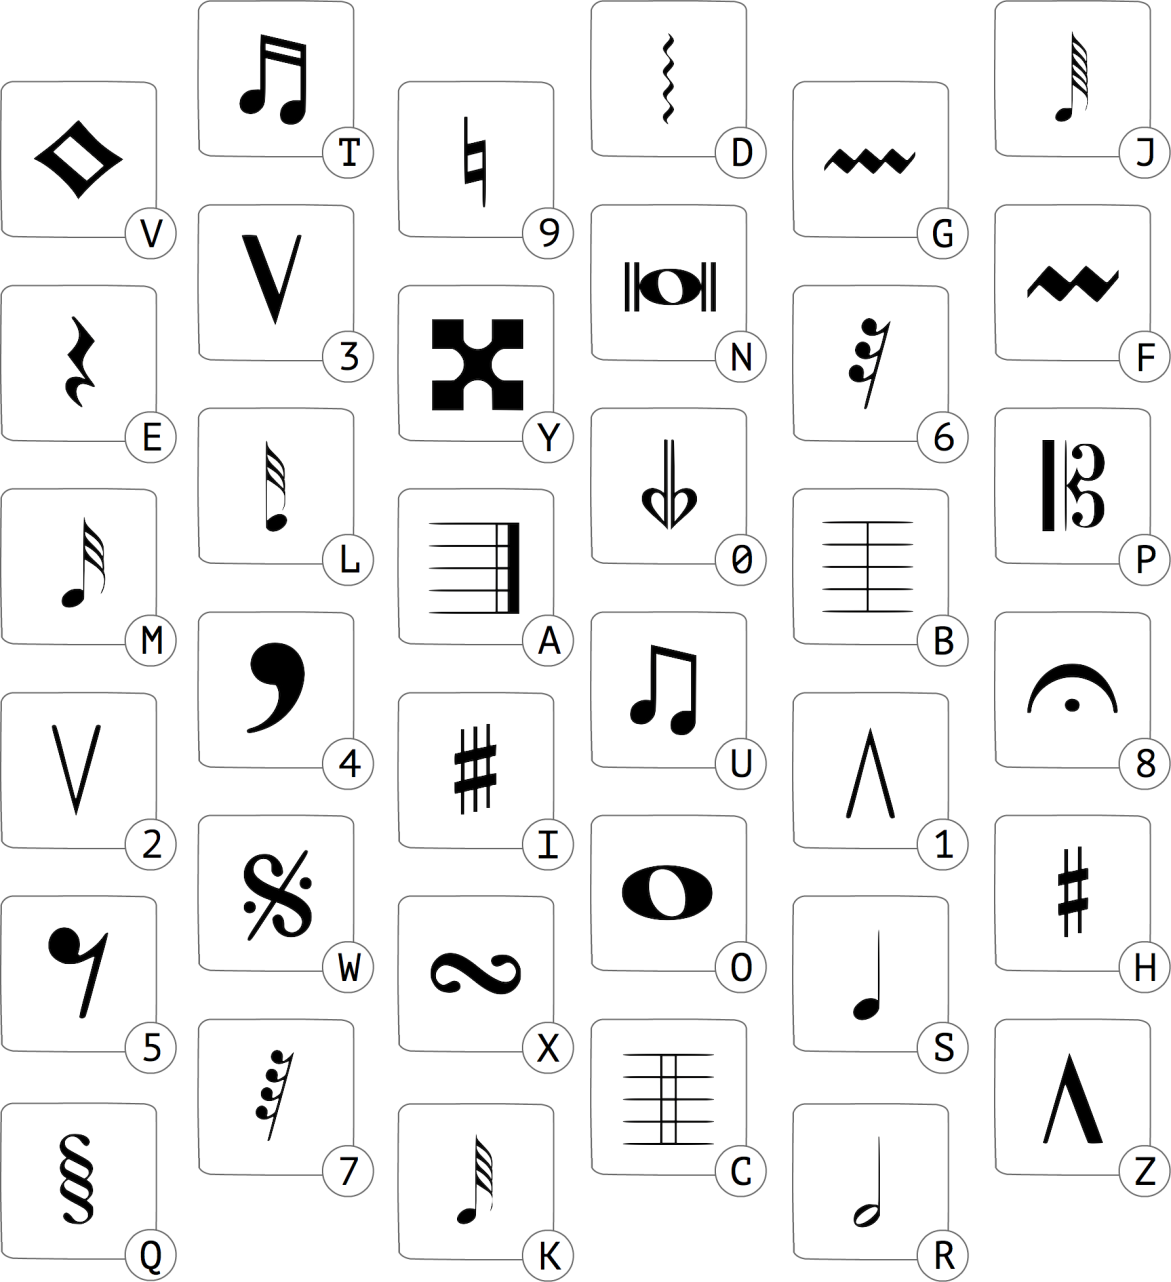
\includegraphics[width=0.85\textwidth]{images/52.png}
\end{center}
